q%%%%%%%%%%%%%%%%%%%%%%%%%%%%%%%%%%%%%%%%%
% University/School Laboratory Report
% LaTeX Template
% Version 3.1 (25/3/14)
%
% This template has been downloaded from:
% http://www.LaTeXTemplates.com
%
% Original author:
% Linux and Unix Users Group at Virginia Tech Wiki 
% (https://vtluug.org/wiki/Example_LaTeX_chem_lab_report)
%
% License:
% CC BY-NC-SA 3.0 (http://creativecommons.org/licenses/by-nc-sa/3.0/)
%
%%%%%%%%%%%%%%%%%%%%%%%%%%%%%%%%%%%%%%%%%

\documentclass{article}

%\usepackage[version=3]{mhchem} % Package for chemical equation typesetting
%\usepackage{siunitx} % Provides the \SI{}{} and \si{} command for typesetting SI units
\usepackage{graphicx} % Required for the inclusion of images
\usepackage{natbib} % Required to change bibliography style to APA
\usepackage{amsmath} % Required for some math elements 
\usepackage{listings}
\lstset{basicstyle=\ttfamily, breaklines=true}
\setlength\parindent{2pt} % Removes all indentation from paragraphs

%\renewcommand{\labelenumi}{\alph{enumi}.} % Make numbering in the enumerate environment by letter rather than number (e.g. section 6)

%\usepackage{times} % Uncomment to use the Times New Roman font


%----------------------------------------------------------------------------------------
%	DOCUMENT INFORMATION
%----------------------------------------------------------------------------------------
\title{Request for Notification - FANS\\ UML for Embedded Systems} % Title

\author{Simone \textsc{Rossi}} % Author name

\date{\today} % Date for the report

\begin{document}

\maketitle % Insert the title, author and date

\begin{center}
\begin{tabular}{l r}
Date Performed: & data \\ % Date the experiment was performed
Partners: & Simone Rossi \\ % Partner names
%& Mary Smith \\
%Instructor: & Professor Smith % Instructor/supervisor
\end{tabular}
\end{center}

% If you wish to include an abstract, uncomment the lines below
% \begin{abstract}
% Abstract text
% \end{abstract}

%----------------------------------------------------------------------------------------
%	SECTION 1
%----------------------------------------------------------------------------------------
NB: all the comments and discussions are related to the extended model which handles also 
message parameters

\section{Hypothesis}
An information is missing: what should the system do if the timer ATST3 expires? I decided to 
inform the air traffic controller via signal. 

\section{Requirements}
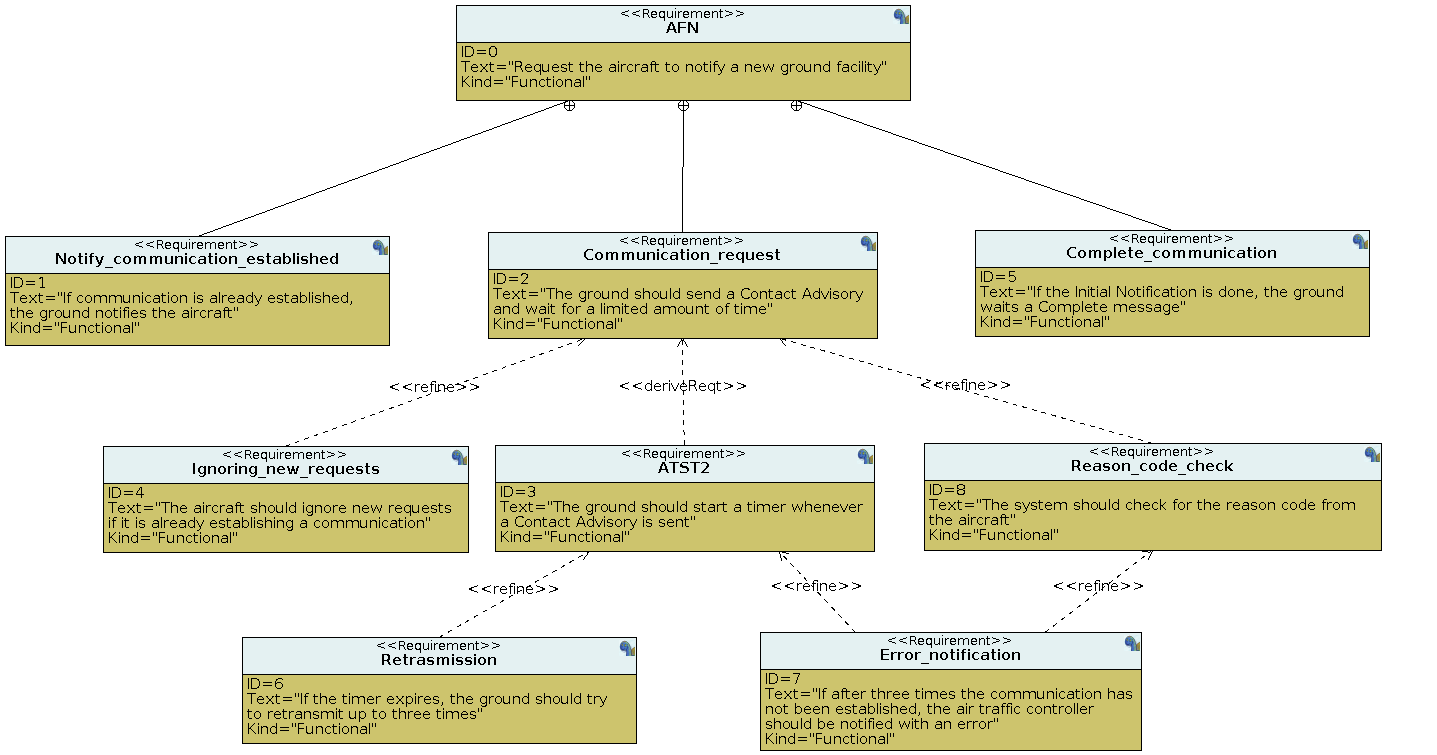
\includegraphics[width=\textwidth]{./lab2_10.png}


\section{Analysis}

\subsection{Case diagram}
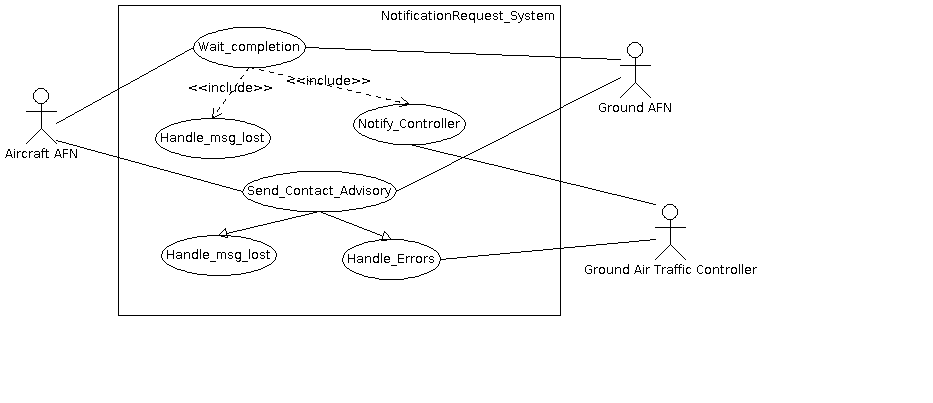
\includegraphics[width=\textwidth]{./lab2_11.png}

\subsection{Nominal Case}
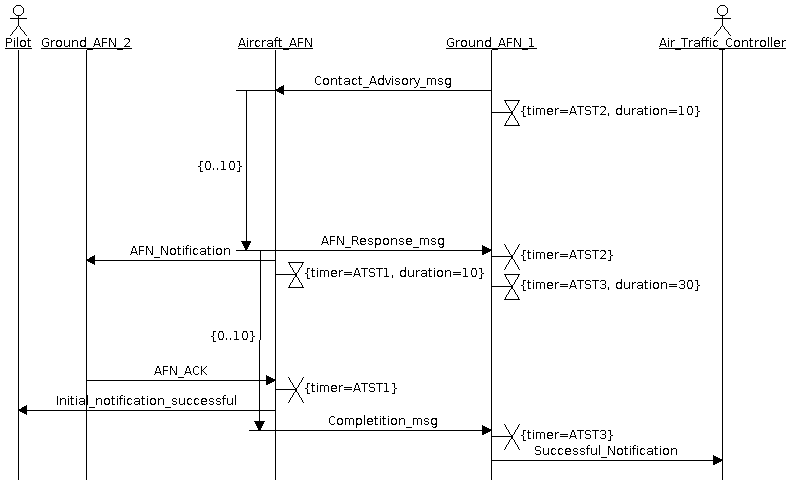
\includegraphics[width=\textwidth]{./lab2_12.png}
Here is shown a nominal case for the Notification Request system. 
The first ground AFN sends to the aircraft the notification to start a new authentication 
procedure with a new facility. As soos as the aircraft receives the message, it replies to
the first AFN and starts the Inital Notification procedure with a new ground AFN. When done,
the pilot as well as the first facility are notified with a successful message. 


\subsection{Error Case 1}
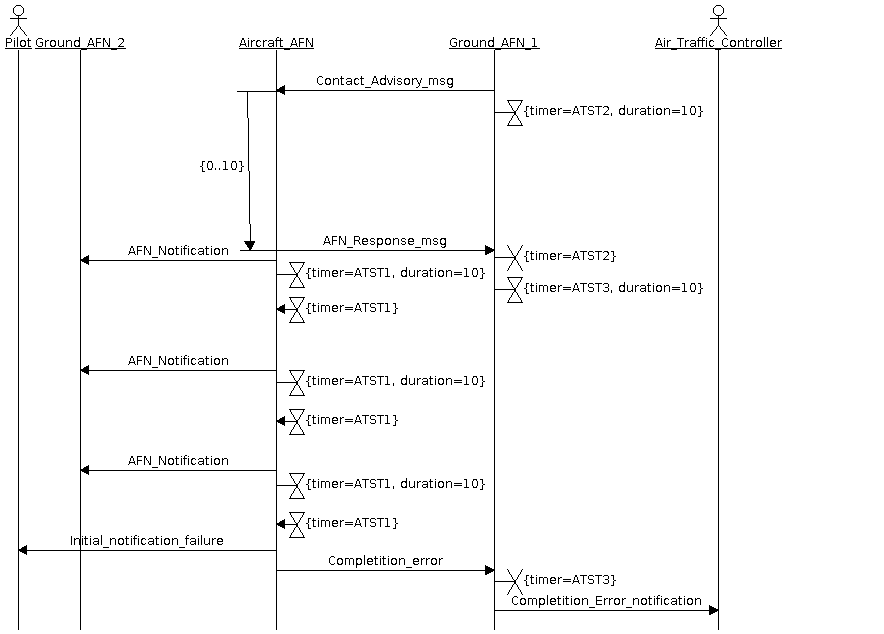
\includegraphics[width=\textwidth]{./lab2_13.png}

\subsection{Error Case 2}
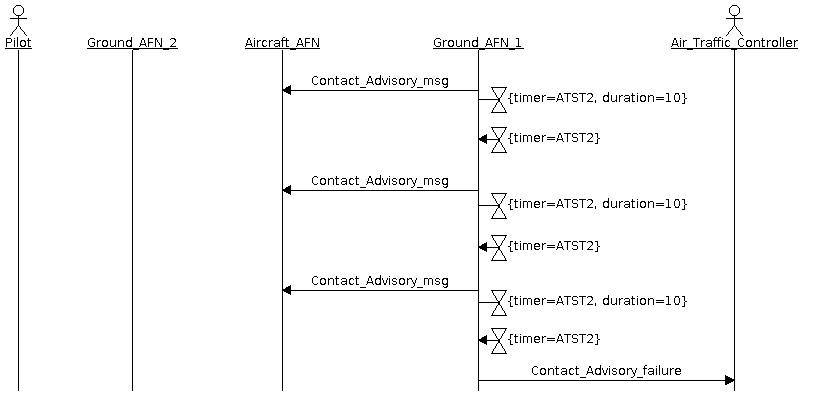
\includegraphics[width=\textwidth]{./lab2_14.png}

\section{Design}

\subsection{Block diagrams}
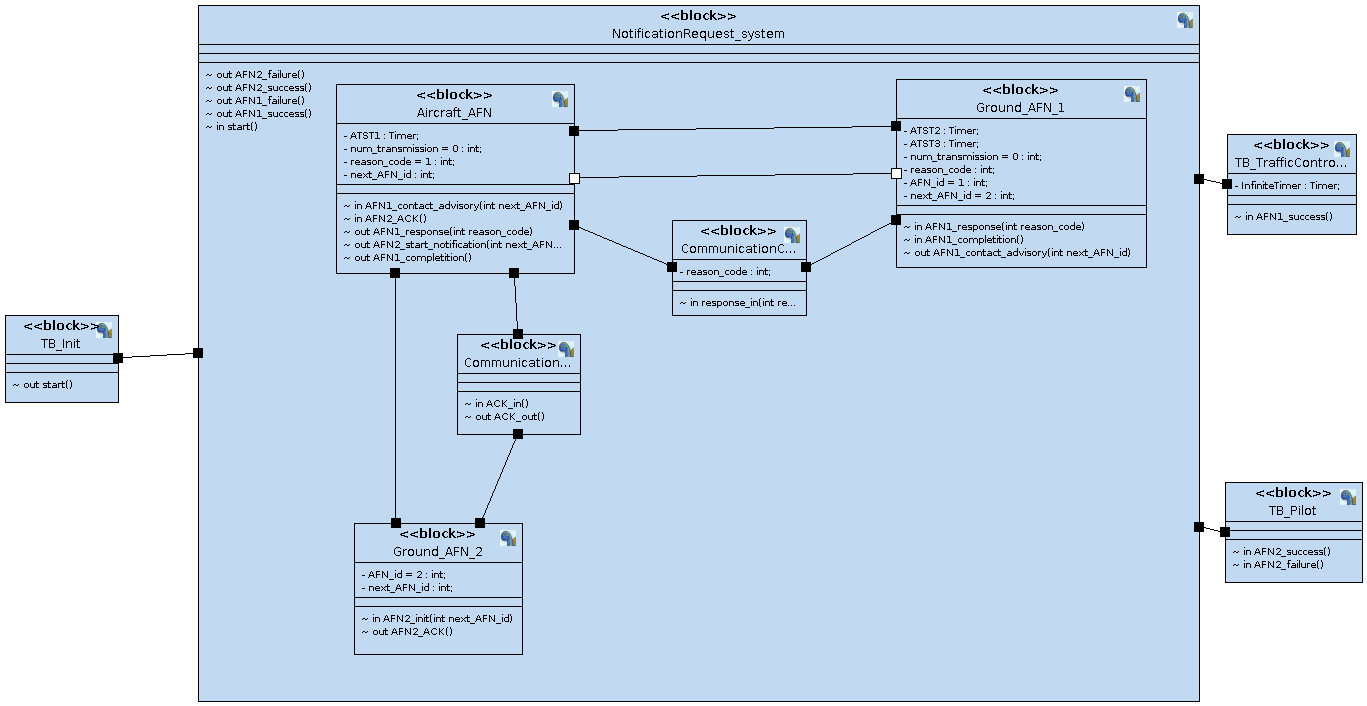
\includegraphics[width=\textwidth]{./lab2_00.png}

\subsection{Flow diagrams}

\subsubsection{Ground AFN1}
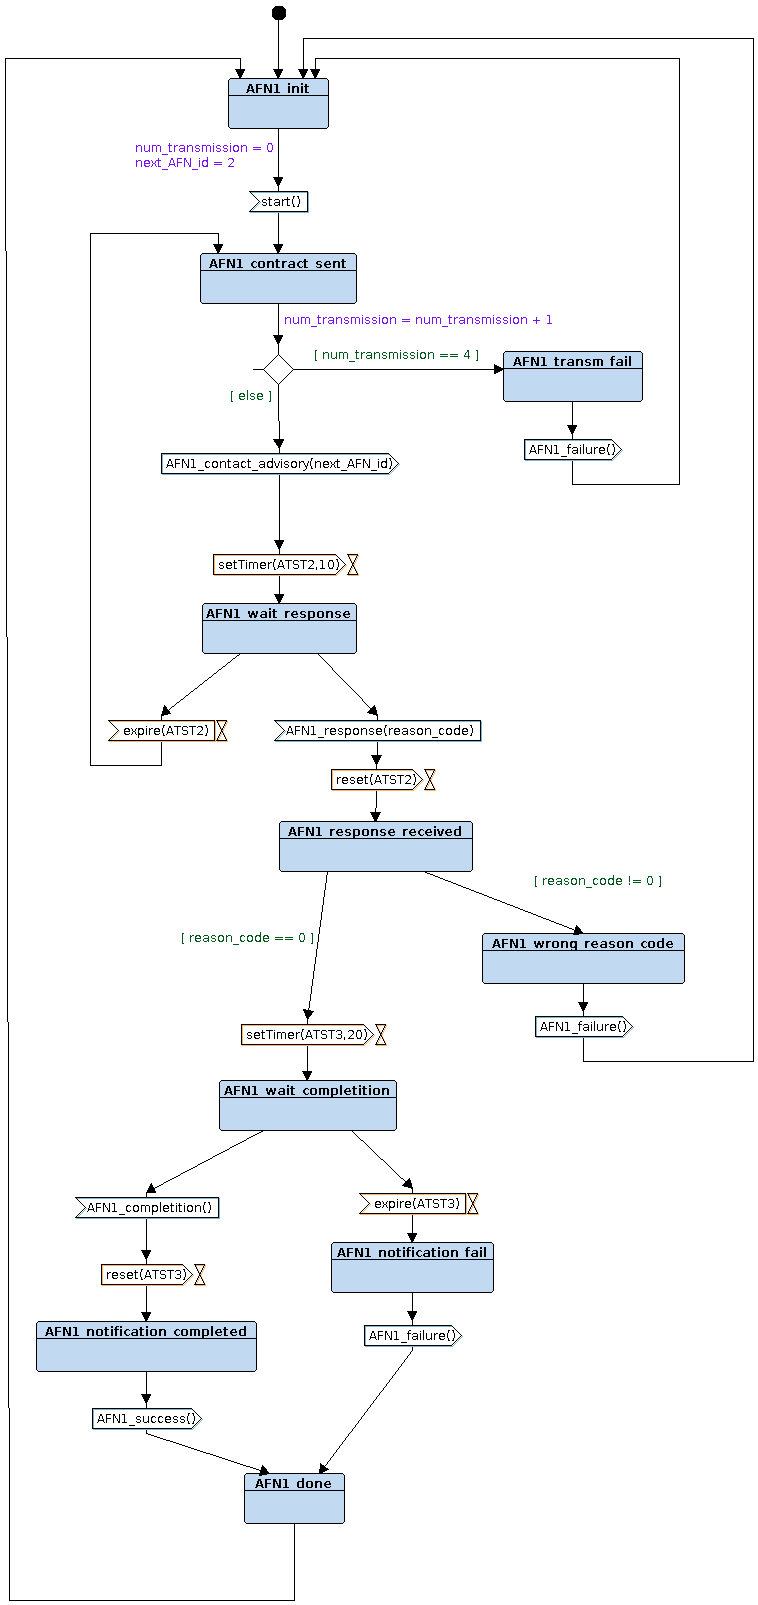
\includegraphics[width=\textwidth]{./lab2_06.png}

\subsubsection{Aircraft AFN}
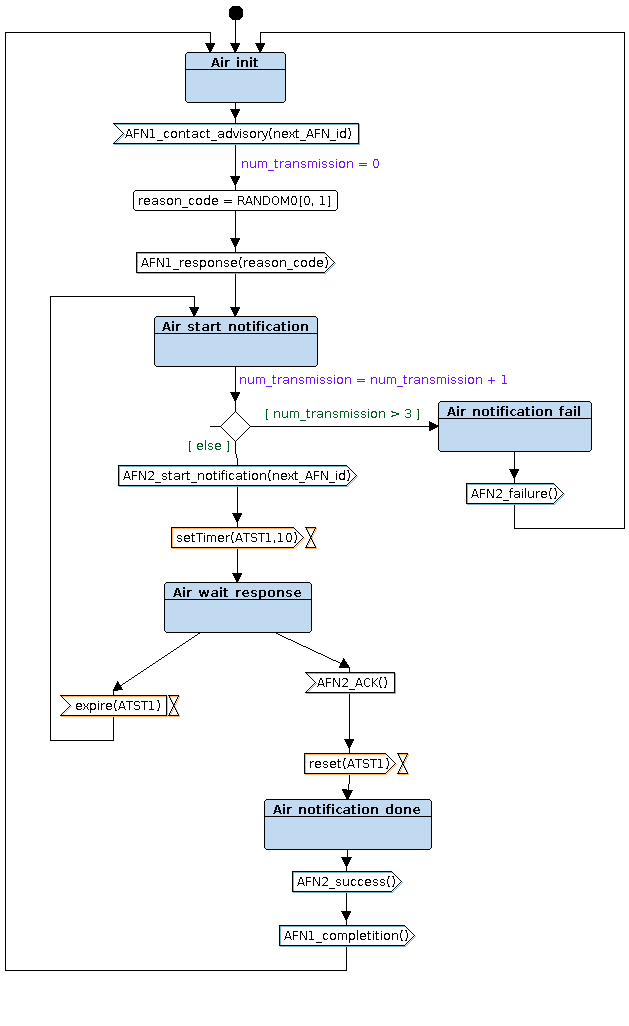
\includegraphics[width=\textwidth]{./lab2_08.png}

\subsubsection{Ground AFN2}
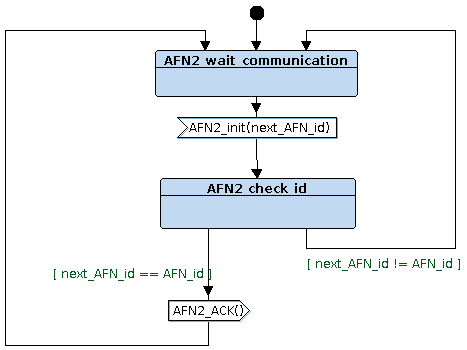
\includegraphics[width=\textwidth]{./lab2_09.png}

\section{Verification}
The reachability and the liveness of the state ``Pilot informed'' and ``Traffic Controller Informed'' are both satisfied. This means that the two actors are always notified whather with a positive or error message. \\
On the other hand, the reachability of the state ``Infinite time'' is not satified: this means that the systems terminate in at most 999 unit of time.  
\end{document}
